%\setcounter{figure}{0} % Manually reset figure count (summary is not a beamer class part)
%\setcounter{framenumber}{0} % Manually reset page count (summary is not a beamer class part)
%\pdfbookmark[1]{Summary of Part II: Reinforcement Learning Using Function Approximation}{Sum_Part_Two} 
\section*{Summary of part II: reinforcement learning using function approximation}  
%\date{}  
%\frame{\titlepage}
\renewcommand{\thefigure}{S-II.\arabic{figure}}  

%%%%%%%%%%%%%%%%%%%%%%%%%%%%%%%%%%%%%%%%%%%%%%%%%%%%%%%%%%%%%
%% Outline / table of content %%
%%%%%%%%%%%%%%%%%%%%%%%%%%%%%%%%%%%%%%%%%%%%%%%%%%%%%%%%%%%%%
\begin{frame}{Table of contents}
	\begin{columns}
		\column{0.5\textwidth}
	  	\begin{varblock}{Summary of part II}
			Reinforcement learning in continuous state and action spaces
	   	\end{varblock}
	\column{0.5\textwidth}
		\small
		  \tableofcontents[hideallsubsections, sections={8-15}]
	\end{columns}
\end{frame}

%%%%%%%%%%%%%%%%%%%%%%%%%%%%%%%%%%%%%%%%%%%%%%%%%%%%%%%%%%%%%
%% What was Covered in the Course %%
%%%%%%%%%%%%%%%%%%%%%%%%%%%%%%%%%%%%%%%%%%%%%%%%%%%%%%%%%%%%%
\frame{\frametitle{What was covered in the course }
\begin{figure}
	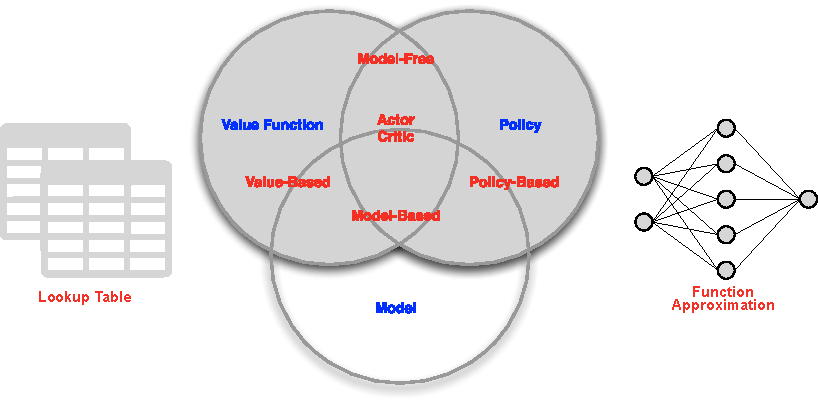
\includegraphics[width=11cm]{fig/lec12/RL_Categories.pdf}
	\caption{Main categories of reinforcement learning algorithms\\  (derived work based on D. Silver, Reinforcement learning, 2016. \href{https://creativecommons.org/licenses/by-nc/4.0}{CC BY-NC 4.0})}
\end{figure}
}

%%%%%%%%%%%%%%%%%%%%%%%%%%%%%%%%%%%%%%%%%%%%%%%%%%%%%%%%%%%%%
%% Additional Topics not Covered in this Course (1) %%
%%%%%%%%%%%%%%%%%%%%%%%%%%%%%%%%%%%%%%%%%%%%%%%%%%%%%%%%%%%%%
\frame{\frametitle{Additional topics not covered in this lecture (1)}
\begin{itemize}
		\item \hl{Structured exploration}: can we find a systematic way for fast and robust exploration?
			\begin{itemize}
		\item \href{https://papers.nips.cc/paper/6591-vime-variational-information-maximizing-exploration.pdf}{R. Houthooft et al., "Vime: Variational information maximizing exploration", Advances in Neural Information Processing Systems, 2016}
		\item \href{http://rail.eecs.berkeley.edu/deeprlcourse/}{S. Levine, CS285 Deep Reinforcement Learning (lecture notes UC Berkeley), 2019}
		\item \href{https://www.davidsilver.uk/wp-content/uploads/2020/03/XX.pdf}{D. Silver, Reinforcement Learning (lecture notes UC London), 2015}
	\end{itemize}\pause
	\vspace{0.5cm}
	\item \hl{Imitation learning}: how can we mimic the behavior of a certain baseline agent / controller / human expert? 
		\begin{itemize}
		\item \href{https://dl.acm.org/doi/pdf/10.1145/3054912}{A. Hussein et al., "Imitation learning: A survey of learning methods", ACM Computing Surveys (CSUR) 50.2, pp. 1-35, 2017}
		\item \href{https://arxiv.org/pdf/1705.10528}{A. Attia and S. Dayan, "Global overview of imitation learning", arXiv:1801.06503, 2018}
	\end{itemize}
\end{itemize}
}

%%%%%%%%%%%%%%%%%%%%%%%%%%%%%%%%%%%%%%%%%%%%%%%%%%%%%%%%%%%%%
%% Additional Topics not Covered in this Course (2) %%
%%%%%%%%%%%%%%%%%%%%%%%%%%%%%%%%%%%%%%%%%%%%%%%%%%%%%%%%%%%%%
\frame{\frametitle{Additional topics not covered in this lecture (2)}
\begin{itemize}
	\item \hl{Multi-agent algorithms}: finding solutions to distributed problems (e.g., for distributed energy systems).
			\begin{itemize}
		\item \href{https://www.researchgate.net/profile/Robert_Babuska/publication/3421909_A_Comprehensive_Survey_of_Multiagent_Reinforcement_Learning/links/02bfe511a5153c4b2c000000/A-Comprehensive-Survey-of-Multiagent-Reinforcement-Learning.pdf}{L. Busoniu, R. Babuska and B. De Schutter. "A comprehensive survey of multiagent reinforcement learning." IEEE Transactions on Systems, Man, and Cybernetics, Part C 38.2, pp. 156-172, 2008 }
		\item \href{https://www.researchgate.net/profile/Pablo_Hernandez-Leal/publication/328280687_Is_multiagent_deep_reinforcement_learning_the_answer_or_the_question_A_brief_survey/links/5d152c8f92851cf440517170/Is-multiagent-deep-reinforcement-learning-the-answer-or-the-question-A-brief-survey.pdf}{P. Hernandez-Leal, B. Kartal and M. Taylor. "Is multiagent deep reinforcement learning the answer or the question? A brief survey", Researchgate preprint, 2018}
	\end{itemize}
	
	\item \hl{Federated learning}: finding solutions to distributed problems via multiple independent sessions, each using its own local information (addressing critical issues such as data privacy, data security, data access rights).
			\begin{itemize}
		\item \href{https://arxiv.org/abs/1901.08277}{H. Zhuo et al. "Federated Deep Reinforcement Learning", arXiv:1901.08277, 2019}
		\item \href{https://arxiv.org/abs/2108.11887}{J. Qi et al. "Federated Reinforcement Learning: Techniques, Applications, and Open Challenges", arXiv:2108.11887, 2021}
	\end{itemize}
\end{itemize}
}

%%%%%%%%%%%%%%%%%%%%%%%%%%%%%%%%%%%%%%%%%%%%%%%%%%%%%%%%%%%%%
%% Learning Summary %%
%%%%%%%%%%%%%%%%%%%%%%%%%%%%%%%%%%%%%%%%%%%%%%%%%%%%%%%%%%%%%
\frame{\frametitle{Learning summary}
\vspace{-0.1cm}
\begin{block}{What you should have learned}
\begin{itemize}
	\item How to model decision processes using a Markov framework. \pause
	\item Finding exact solutions using iterative tabular methods for discrete problem spaces.  \pause
	\item Finding approximate solutions for large discrete or continuous problem spaces based on function approximation.  \pause
	\item Application of just these techniques on a practical programming level.\pause
\end{itemize}
\end{block}
\begin{block}{Concluding remarks}
\begin{itemize}
	\item This is an introductory course to RL. We have only scratched the surface. \pause
	\item Some aspects, especially within the exercises, had a control focus. In other application, specific RL solutions can look quite different.  \pause
	\item If you are interested in more practical RL insights in the field of electrical power systems, do not hesitate to contact us.
\end{itemize}
\end{block}
}

\renewcommand{\thefigure}{\arabic{section}.\arabic{figure}}